%!TEX root = ../Thesis.tex
\chapter{Pendulum - Hamilton's Equations and Numerical Analysis}


\section{Equations of Motion}
\begin{figure}[ht!]
\centering 
\includegraphics[scale=1.2]{fig/pendulum.pdf}
\caption{The pendulum}
\label{fig:pe}
\end{figure}
\begin{description}
\item[Step 0 \quad Lagrangian $L$] \ \\[0.5cm]
Generalized coordinate: $\theta$. \\[0.2cm]
$T = \frac{1}{2} m \dot{x}^2 = \frac{1}{2} m l^2 \theta^2.$ \\[0.2cm]
$V = -m g l \cos{\theta}$ \\[0.2cm]
$L(\theta, \dot{\theta}) = T - V = \frac{1}{2} m l^2 \theta^2 + m g l \cos{\theta}$

\item[Step 1 \quad Generalized momentum $p_\theta$] \ \\[0.2cm]
$p_\theta(\theta,\dot{\theta}) = \dfrac{\partial L}{\partial \dot{\theta}} = m l^2 \dot{\theta}$

\item[Step 2 \quad Transform $\dot{\theta}$] \ \\[0.5cm]
$\dot{\theta} = \dot{\theta}(\theta, p_\theta) = \dfrac{p_\theta}{m l^2}$

\item[Step 3 \quad The Hamiltonian $H$] \ \\[0.5cm]
$H(\vec{q}, \vec{p}, t) = \sum\limits_{i=1}^n p_i \dot{q_i} - L$ \\[0.5cm]
\begin{align}
\nonumber H &= p_\theta \dot{\theta} - \left(\dfrac{1}{2} m l^2 \dot{\theta}^2 + m g l \cos{\theta}\right) \\
\nonumber &= p_\theta \left(\dfrac{p_\theta}{m l^2} \right) - \left(\dfrac{1}{2} m l^2 \left(\dfrac{p_\theta}{m l^2}\right)^2 + m g l \cos{\theta}\right) \\
&= \dfrac{p_\theta^2}{2 m l^2} - m g l \cos{\theta}
\end{align} 
, which we again recognize simply as the total energy. The first term is the kinetic energy in terms of the momentum $p_\theta$ and the second term is the potential energy $V$.

\item[Step 4 \quad Hamilton's Equations of Motion]
\begin{align}
\begin{split}
\label{eq:pe-eom}
\dot{\theta} = +\dfrac{\partial H}{\partial p_\theta} &= \dfrac{p_\theta}{m l^2} ,
\\[0.2cm]
\dot{p_\theta} = -\dfrac{\partial H}{\partial \theta} &= - m g l \sin{\theta}
\end{split}
\end{align}
\end{description}


\section{Numerical Analysis}
We will now solve the pendulum's equations of motion, \eqref{eq:ho-eom}. For simplicity we'll set $k = m = 1$. Note that by choice of $m=l=1$, the momentum $p_\theta$ is actually equal to the angular velocity $\omega$. The first step is to discretize the equations
\begin{alignat}{2}
&\dod{\theta}{t} = p  & \qquad \implies \qquad &\Delta \theta = p \Delta t \\[0.5cm]
&\dod{p}{t} = -\sin{\theta} & \qquad \implies \qquad &\Delta p = - \sin{\theta} \Delta t
\end{alignat}
This is a non-linear system of PDEs with no analytical solution. The small angle approximation $\sin{\theta} = \theta$ makes this system identical to the harmonic oscillator. However we're interested in solving the exact system where large oscillations are permitted. We will not be able to compare our numerical solutions to an analytical one (since none exists), but we can gain valuable insights nonetheless.

Once again, in the explicit Euler use old time step values $i$, implicit Euler use new time step values $i+1$ and the symplectic Euler use mixed time step values. As we will see, now the implicit Euler necessitates finding roots numerically.
\subsection{Explicit Euler algorithm}
\begin{align}
\begin{split}
\label{al:pe-euler_e}
\theta_{i+1} &= p_i \Delta t + \theta_i \\
p_{i+1} &= - \sin{\theta_i} \Delta t + p_i
\end{split}
\end{align}

\subsection{Implicit Euler algorithm}
\begin{align}
\begin{split}
\label{al:pe-euler_i}
\theta_{i+1} &= p_{i+1} \Delta t + \theta_i \\
p_{i+1} &= - \sin{\theta_{i+1}} \Delta t + p_i
\end{split}
\end{align}
The new time step $i+1$ values are then found by substituting on the the equations into the other, then solving numerically with a root finder algorithm. For example we can substitute the expression for $p_{i+1}$ into $\theta_{i+1}$ and solve the resulting equation
\begin{align}
0 = \theta_i - \theta_{i+1} + (p_i - sin{\theta_{i+1}})\Delta t
\end{align}
Now run root finding for $\theta_{i+1}$, guessing $\theta_i$ as initial guess.

\subsection{Symplectic Euler algorithm}
\begin{align}
\begin{split}
\label{al:pe-euler_s1}
\theta_{i+1} &= p_{i+1} \Delta t + \theta_i \\
p_{i+1} &= - \sin{\theta_i} \Delta t + p_i
\end{split}
\end{align}
or
\begin{align}
\begin{split}
\label{al:pe-euler_s2}
\theta_{i+1} &= p_{i} \Delta t + \theta_i \\
p_{i+1} &= - \sin{\theta_{i+1}} \Delta t + p_i
\end{split}
\end{align}
Algorithms \crefrange{al:pe-euler_e}{al:pe-euler_s1} was implemented in Python (Appendix \ref{app:pe}).

\section{Plots}
\begin{figure}
    \centering
        \subbottom[Explicit Euler]{
            \includegraphics[scale=0.24]{fig/pe/pe_y(x)_euler_explicit.pdf}
            \label{fig:pe_y(x)_euler_explicit}
        }
        \subbottom[Implicit Euler]{
            \includegraphics[scale=0.24]{fig/pe/pe_y(x)_euler_implicit.pdf}
            \label{fig:pe_y(x)_euler_implicit}
        }
        \subbottom[Symplectic Euler]{
            \includegraphics[scale=0.24]{fig/pe/pe_y(x)_euler_symplectic.pdf}
            \label{fig:pe_y(x)_euler_symplectic}
        }
        \caption{Position y(x)}
    \label{fig:pe_y(x)_euler}
\end{figure}

\begin{figure}
    \centering
        \subbottom[Explicit Euler]{
            \includegraphics[scale=0.24]{fig/pe/pe_omega(t)_euler_explicit.pdf}
            \label{fig:pe_omega(t)_euler_explicit}
        }
        \subbottom[Implicit Euler]{
            \includegraphics[scale=0.24]{fig/pe/pe_omega(t)_euler_implicit.pdf}
            \label{fig:pe_omega(t)_euler_implicit}
        }
        \subbottom[Symplectic Euler]{
            \includegraphics[scale=0.24]{fig/pe/pe_omega(t)_euler_symplectic.pdf}
            \label{fig:pe_omega(t)_euler_symplectic}
        }
        \caption{Momentum p(t), equivalent to angular velocity $\omega(t)$ by choice of $m=l=1$}
    \label{fig:pe_omega(t)_euler}
\end{figure}

\begin{figure}
    \centering
        \subbottom[Explicit Euler]{
            \includegraphics[scale=0.24]{fig/pe/pe_E(t)_euler_explicit.pdf}
            \label{fig:pe_E(t)_euler_explicit}
        }
        \subbottom[Implicit Euler]{
            \includegraphics[scale=0.24]{fig/pe/pe_E(t)_euler_implicit.pdf}
            \label{fig:pe_E(t)_euler_implicit}
        }
        \subbottom[Symplectic Euler]{
            \includegraphics[scale=0.24]{fig/pe/pe_E(t)_euler_symplectic.pdf}
            \label{fig:pe_E(t)_euler_symplectic}
        }
        \caption{Energy E(t), note y-scale on \ref{fig:pe_E(t)_euler_symplectic}}
    \label{fig:pe_E(t)_euler}
\end{figure}

\begin{figure}
    \centering
        \subbottom[Explicit Euler]{
            \includegraphics[scale=0.24]{fig/pe/pe_phase-space_euler_explicit.pdf}
            \label{fig:pe_phase-space_euler_explicit}
        }
        \subbottom[Implicit Euler]{
            \includegraphics[scale=0.24]{fig/pe/pe_phase-space_euler_implicit.pdf}
            \label{fig:pe_phase-space_euler_implicit}
        }
        \subbottom[Symplectic Euler]{
            \includegraphics[scale=0.24]{fig/pe/pe_phase-space_euler_symplectic.pdf}
            \label{fig:pe_phase-space_euler_symplectic}
        }
        \caption{Phase-space $p(\theta) = \omega(\theta)$}
    \label{fig:pe_phase-space_euler}
\end{figure}
Things to note this time from the figures \crefrange{fig:pe_y(x)_euler}{fig:pe_phase-space_euler}:
\begin{itemize}
    \item The initial conditions are set such that the pendulum barely has enough energy to go all the way around. Hence the implicit Euler method, known for loosing energy, does not make it all the way around, see fig \ref{fig:pe_y(x)_euler_implicit} as opposed to the explicit and symplectic, fig \ref{fig:pe_y(x)_euler_explicit} and \ref{fig:pe_y(x)_euler_symplectic}.
    \item Symplectic once again keeps the energy $E(t)$ almost constant, and conserves it seemingly perfectly on average over a cycle.
    \item The implicit Euler is in a closed orbit in the phase-space diagram as expected from the position plot \ref{fig:pe_y(x)_euler_implicit}, but spirals inward as expected from the energy plot \ref{fig:pe_E(t)_euler_implicit}, whereas explicit and symplectic steadily increases their angles from the initial angle.
\end{itemize}
To summarize, we have seen that the symplectic version of the Euler method for numerical integration is superior because it conserves the quantity that we most care about the reduced 3-body system: energy. In more general terms symplectic integrators conserves the Hamiltonian $H$, which in our cases is the same is the total energy $E$ as discussed in the chapter on using Hamiltonian mechanics. Using symplectic Euler going forward, we are now ready to solve the restricted 3-body problem.